\chapter{基于特征融合和注意力机制的端到端运动想象脑电图分类网络}

上一章提出的DIS-Net模型基于多尺度密集连接和局部混合注意力构建,能够有效地捕获EEG信号的局部特征,然而,仍然存在缺乏全局依赖信息的问题。本章针对EEG信号的时序特性,使用LSTM获取长短期时序依赖,同时,构建了全局自注意力模块SCoT以更好地利用EEG信号的全局时空信息,构建出一种能够有效捕获长距离依赖信息的模型LS-Net。为了同时利用EEG信号的局部特征细节和全局依赖信息,实现更为丰富的特征融合效果,论文将DIS-Net与LS-Net提取的特征进行融合,构建出最终模型HA-FuseNet,获得更好的MI-EEG分类效果。

\section{基于特征融合和注意力机制的端到端MI-EEG分类网络HA-FuseNet}

原始的EEG信号通常为二维数据,包括通道(电极)和时间两个维度,具体而言,在EEG信号矩阵中,行代表分布在头皮不同位置的采样通道,列为时间序列数据,每个采样点对应一个时间戳下的生物电信号(通常为电压值),因此,一列数据就是一个特定时间点下所有通道同步采集到的电压读数。原始的EEG信号经过预处理之后,可以转换为时频图、头皮点位拓扑图等输入模式,尽管经过转换的输入相较于原始输入能够更全面地体现EEG信号的时频空信息,但这一过程往往需要具有神经科学背景的人工参与,在增加了人工成本同时,限制了模型自适应学习EEG信号中蕴含的复杂时空特征的能力,此外,复杂的预处理环节也增加了计算开销和应用成本,难以满足BCI系统即时响应的需求。因此,端到端网络在MI-EEG分类领域受到越来越多的重视,这类网络不经过或者仅仅经过很少的预处理步骤,而由深度学习算法自适应地提取关键特征并作出预测。

为此,论文最终构建了一种基于特征融合和注意力机制的端到端MI-EEG分类网络HA-FuseNet,其结构如图~\ref{fig:hafuse}~所示。HA-FuseNet通过两个子网络分别进行特征提取,随后进行特征融合和最终的分类预测。两个子网络分别是基于卷积神经网络搭建的DIS-Net与基于长短期记忆网络的LS-Net。其中,DIS-Net用于局部特征的提取,LS-Net则提供了全局时空长距离依赖信息,因此,将DIS-Net和LS-Net提取的特征进行融合,能够取长补短,在利用卷积神经网络提取到的局部信息的同时有效地建立全局依赖关系,从而获取更为精准的分类效果。

DIS-Net为前一章构建的模型,其通过Inception结合密集连接的多尺度密集连接模块,进行多尺度特征提取,同时利用高级语义信息与浅层特征;通过引入反转瓶颈层,在深度维度上促进时空特征的融合;通过引入svSE混合注意力模块促进网络对重要特征的关注度,svSE模块采取时空特征分离的策略,同时利用了EEG信号的方差信息,以获得针对性的结果。LS-Net用以获取时空域的长期依赖信息,通过LSTM获取时间域的长短期依赖信息,并且加入了SCoT全局注意力模块获取时空域的全局上下文信息。两个子网络通过C2R模块和R2C模块进行交互,并在深度维度进行特征的融合。在特征融合之后,通过使用了深度可分离卷积的空间卷积层,在提取空间特征的同时减少计算消耗,最后,通过全连接层进行分类的预测。通过HA-FuseNet,可以更完整地获取MI-EEG信号的有效特征,提升分类的效果。
\begin{figure}
    \centering
    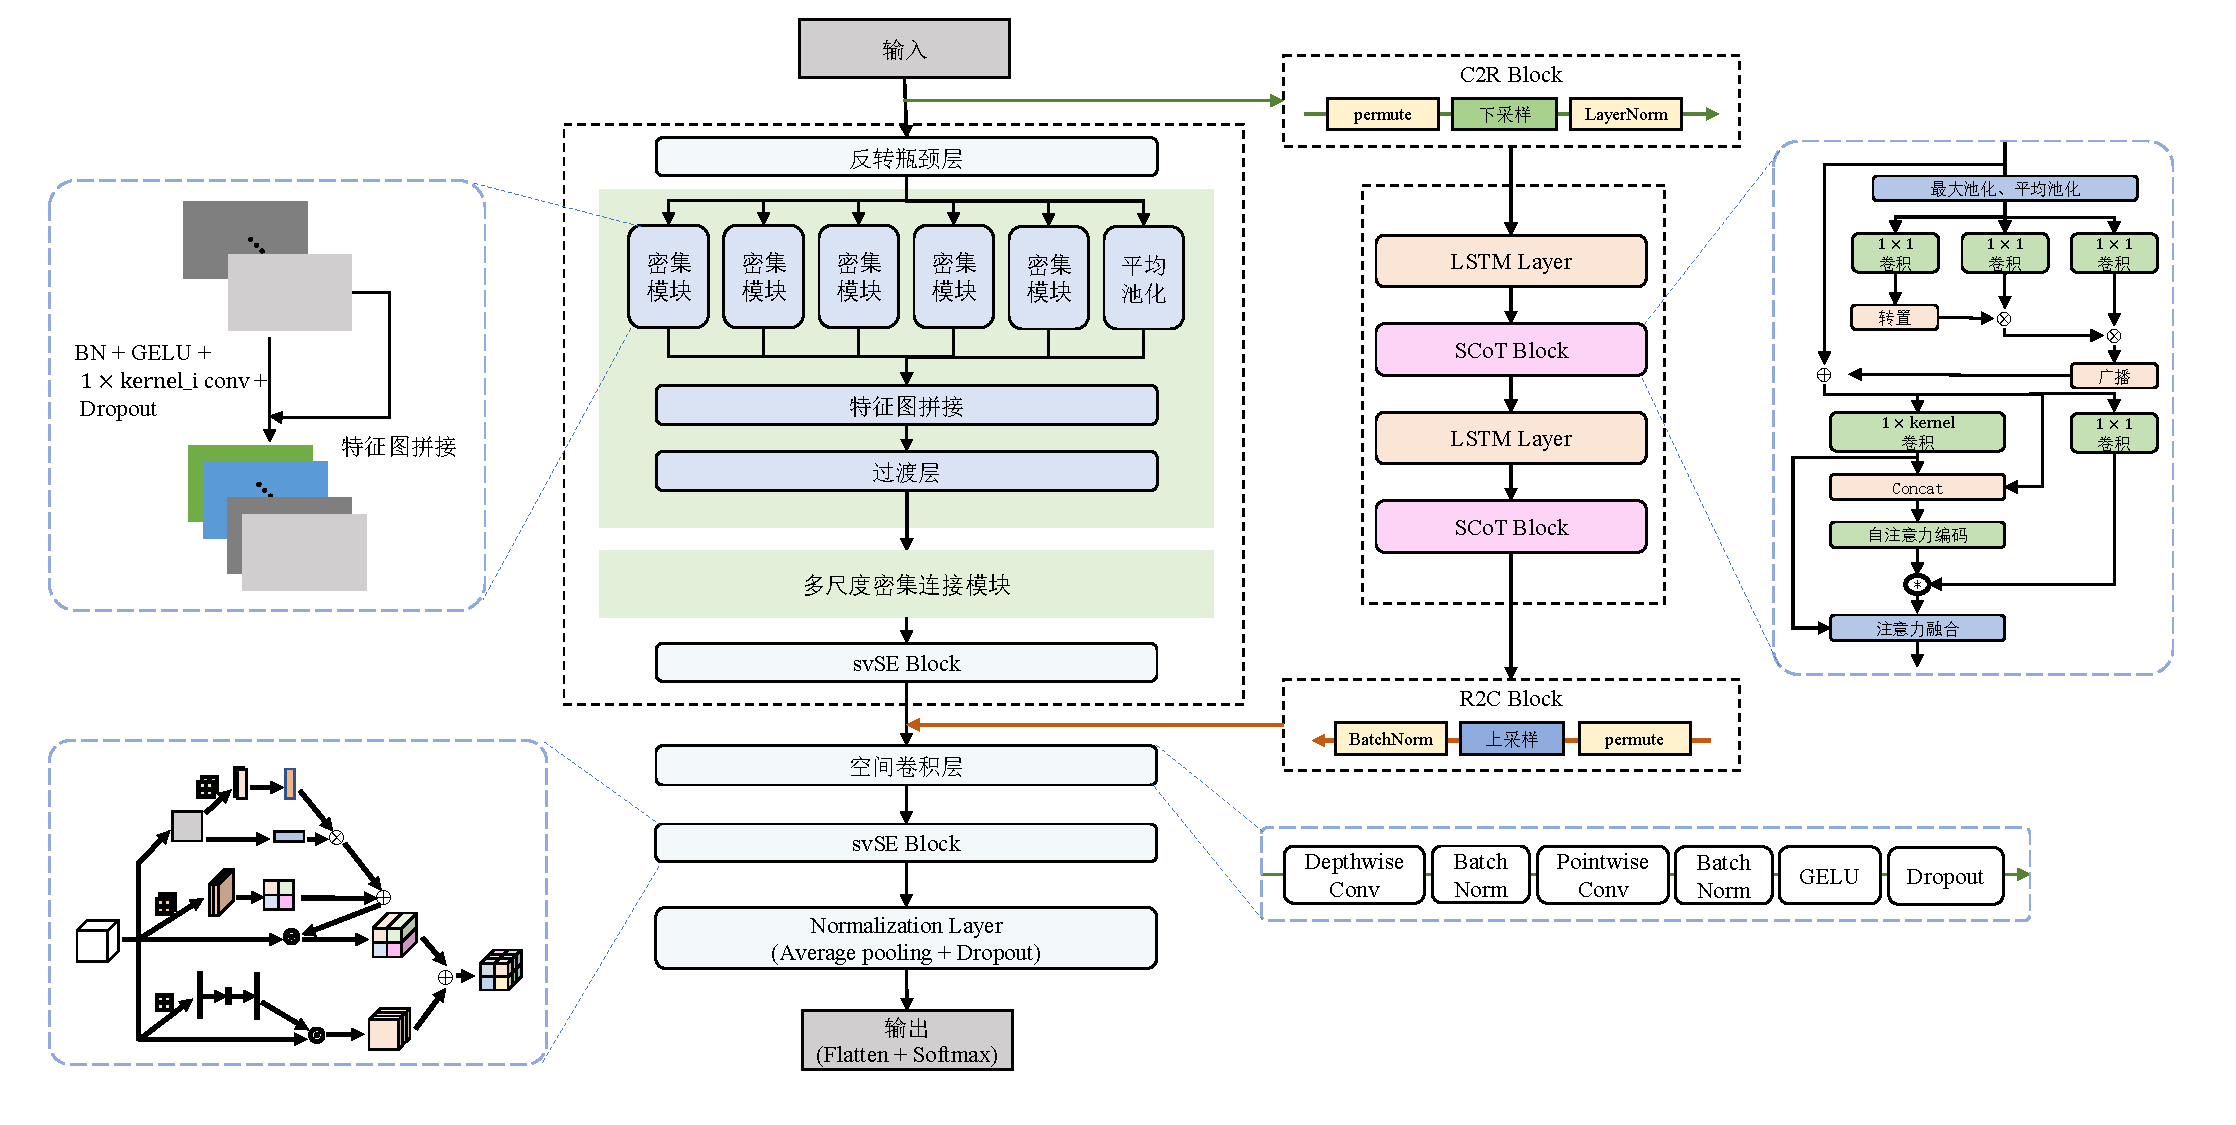
\includegraphics[width=\textwidth]{HA-FuseNetv2.pdf}
    \caption{HA-FuseNet结构}
    \label{fig:hafuse}
\end{figure}

% \section{基于多尺度密集连接和局部注意力的分类网络DIS-Net}

% 即论文在第三章构建的模型,此处不再赘述。

\section{结合全局自注意力的分类网络}

卷积神经网络倾向于模拟人类视觉系统,卷积层具有局部感受野,能够出色地捕获信号中的局部时空特征,但对于那些跨越较长时间跨度和空间分布的复杂交互信息,其建模能力受限。EEG信号作为随时间变化的信号,具有时间序列属性,长短期记忆网络能够捕获时间域的长期依赖,适合处理序列数据,但缺乏对空间信息进行提取的能力。为此,论文选择LSTM结合全局自注意力的方式,为模型加入全局时空信息。

\subsection{全局自注意力SCoT}

LSTM能够一定程度上捕获序列数据的长期依赖关系,但EEG信号在具有长距离时间依赖的同时具有全局空间特性,使得LSTM无法充分挖掘并整合全局时空域的依赖信息。因此,论文基于Non-local\cite{wang2018non}和Contextual Transformer(CoT)\cite{li2022contextual}这两种全局自注意力机制进行改进,针对EEG信号的特点提出了SCoT(Separate Contextual Transformer)模块,旨在更完整地捕捉EEG信号在时空域内的全局依赖关系,从而增强模型的全局建模能力。

Non-local是将自注意力\cite{vaswani2017attention}应用于计算机视觉领域的一项经典模型,能够捕捉特征图中任意两个位置之间的依赖关系,其结构如图~\ref{fig:non-local}~所示。对于输入\(X \in \mathbb{R}^{C \times H \times W}\),首先通过三个\(1\times1\)卷积将通道数量由\(C\)压缩为\(\frac{C}{2}\),分别得到代表查询、键和值矩阵的三个特征图\(X_\theta\)、\(X_\phi\)和\(X_g\)。随后对\(X_\theta\)、\(X_\phi\)、\(X_g\)进行展平(Flatten),并通过点积操作计算\(X_\theta\)与\(X_\phi\)的相似度矩阵\(S\),该矩阵代表输入特征图中各个位置之间的联系。接着,使用Softmax函数对相似度矩阵\(S\)进行归一化,使得其转化为概率分布,并与值矩阵\(X_g\)相乘,得到结果矩阵\(Y \in \mathbb{R}^{\frac{C}{2} \times H \times W}\),最后,通过\(1\times1\)卷积恢复\(Y\)的维度至与\(X\)相同,以逐元素相加的方式得到加权后的结果。Non-local通过直接计算两个位置之间的远程依赖关系,能够获取全局自注意力,但在数据量较大的情况下,存在计算量偏大的问题。

CoT考虑到Non-local忽略了相邻键上下文信息的问题,提出了一种将上下文信息挖掘能力集成入自注意力机制中的方式,其结构如图~\ref{fig:cot}~所示。对于输入\(X \in \mathbb{R}^{C \times H \times W}\),CoT的改动主要在于使用\(3\times3\)卷积获取特征图的静态上下文信息,将其作为键矩阵\(K\),同时,通过\(1\times1\)卷积获取到值矩阵\(V\),直接获取了查询矩阵\(Q\),然后对\(K\)和\(Q\)进行深度维度的聚合,并通过两个连续的\(1\times1\)卷积获取注意力权重图\(A\),通过注意力权重图\(A\)和值矩阵\(V\)相乘获取特征图的动态上下文信息,最后将静态上下文信息和动态上下文信息进行了融合。
\begin{figure}[ht]
  \centering
  \begin{subfigure}{0.4\textwidth}
    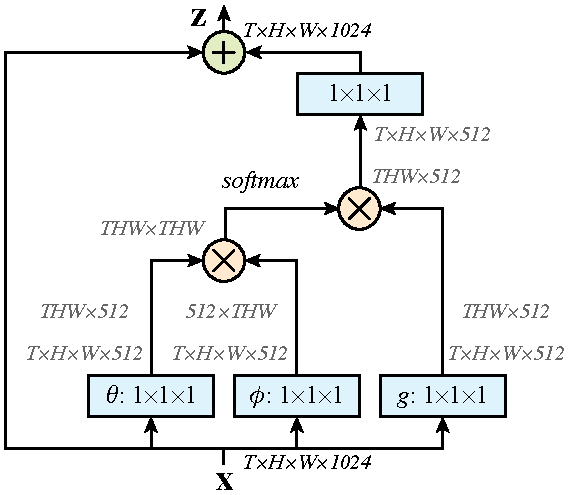
\includegraphics[width=\linewidth]{non-local.pdf}
    \caption{Non-local结构\cite{wang2018non}}
    \label{fig:non-local}
  \end{subfigure}\qquad
  \begin{subfigure}{0.4\textwidth}
    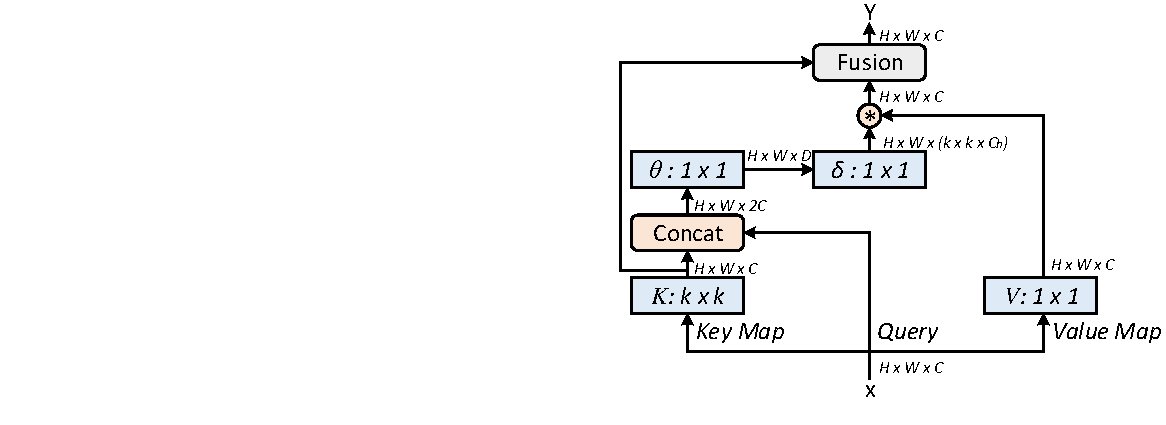
\includegraphics[width=\linewidth]{cot.pdf}
    \caption{CoT结构\cite{li2022contextual}}
    \label{fig:cot}
  \end{subfigure}
  \caption{两种全局自注意力}
  \label{fig:self}
\end{figure}

对于运动想象MI-EEG分类任务来说,问题在于EEG信号的特性:EEG信号的时域和空域具有较低的局部相关性;在空域上,尽管相邻的电极具有空间相关性,但在EEG原始输入中,相邻的电极未必排列为相邻的通道,因此,在端到端网络的情况下,空域内具有较低的局部相关性;在时域上,EEG信号具有局部相关性,即相邻的采样点往往蕴含相似的信息。因此,Non-local模块和CoT模块无法直接迁移至运动想象MI-EEG分类任务中:Non-local模块能够计算任意两个位置之间的远程依赖关系,但在较大的数据量下,其计算代价高昂;而CoT模块则是基于图像数据的局部相关性,将局部上下文信息引入了自注意力机制中,并通过卷积操作减少了计算量。论文借鉴Non-local和CoT的思想,提出了SCoT模块。

综合考量EEG信号的时空特性与Non-local、CoT各自的特点,论文提出的SCoT注意力模块采取了时空域分步计算全局自注意力的策略,具体来说,针对空域中局部相关性较弱且数据规模有限的情况,对Non-local模块进行改良以适应空间自注意力计算;而对于具有强局部相关性且数据规模较大的时域信息,基于CoT进行改进以计算时间自注意力。SCoT的结构如图~\ref{fig:gsa}~所示。
\begin{figure}[ht]
    \centering
    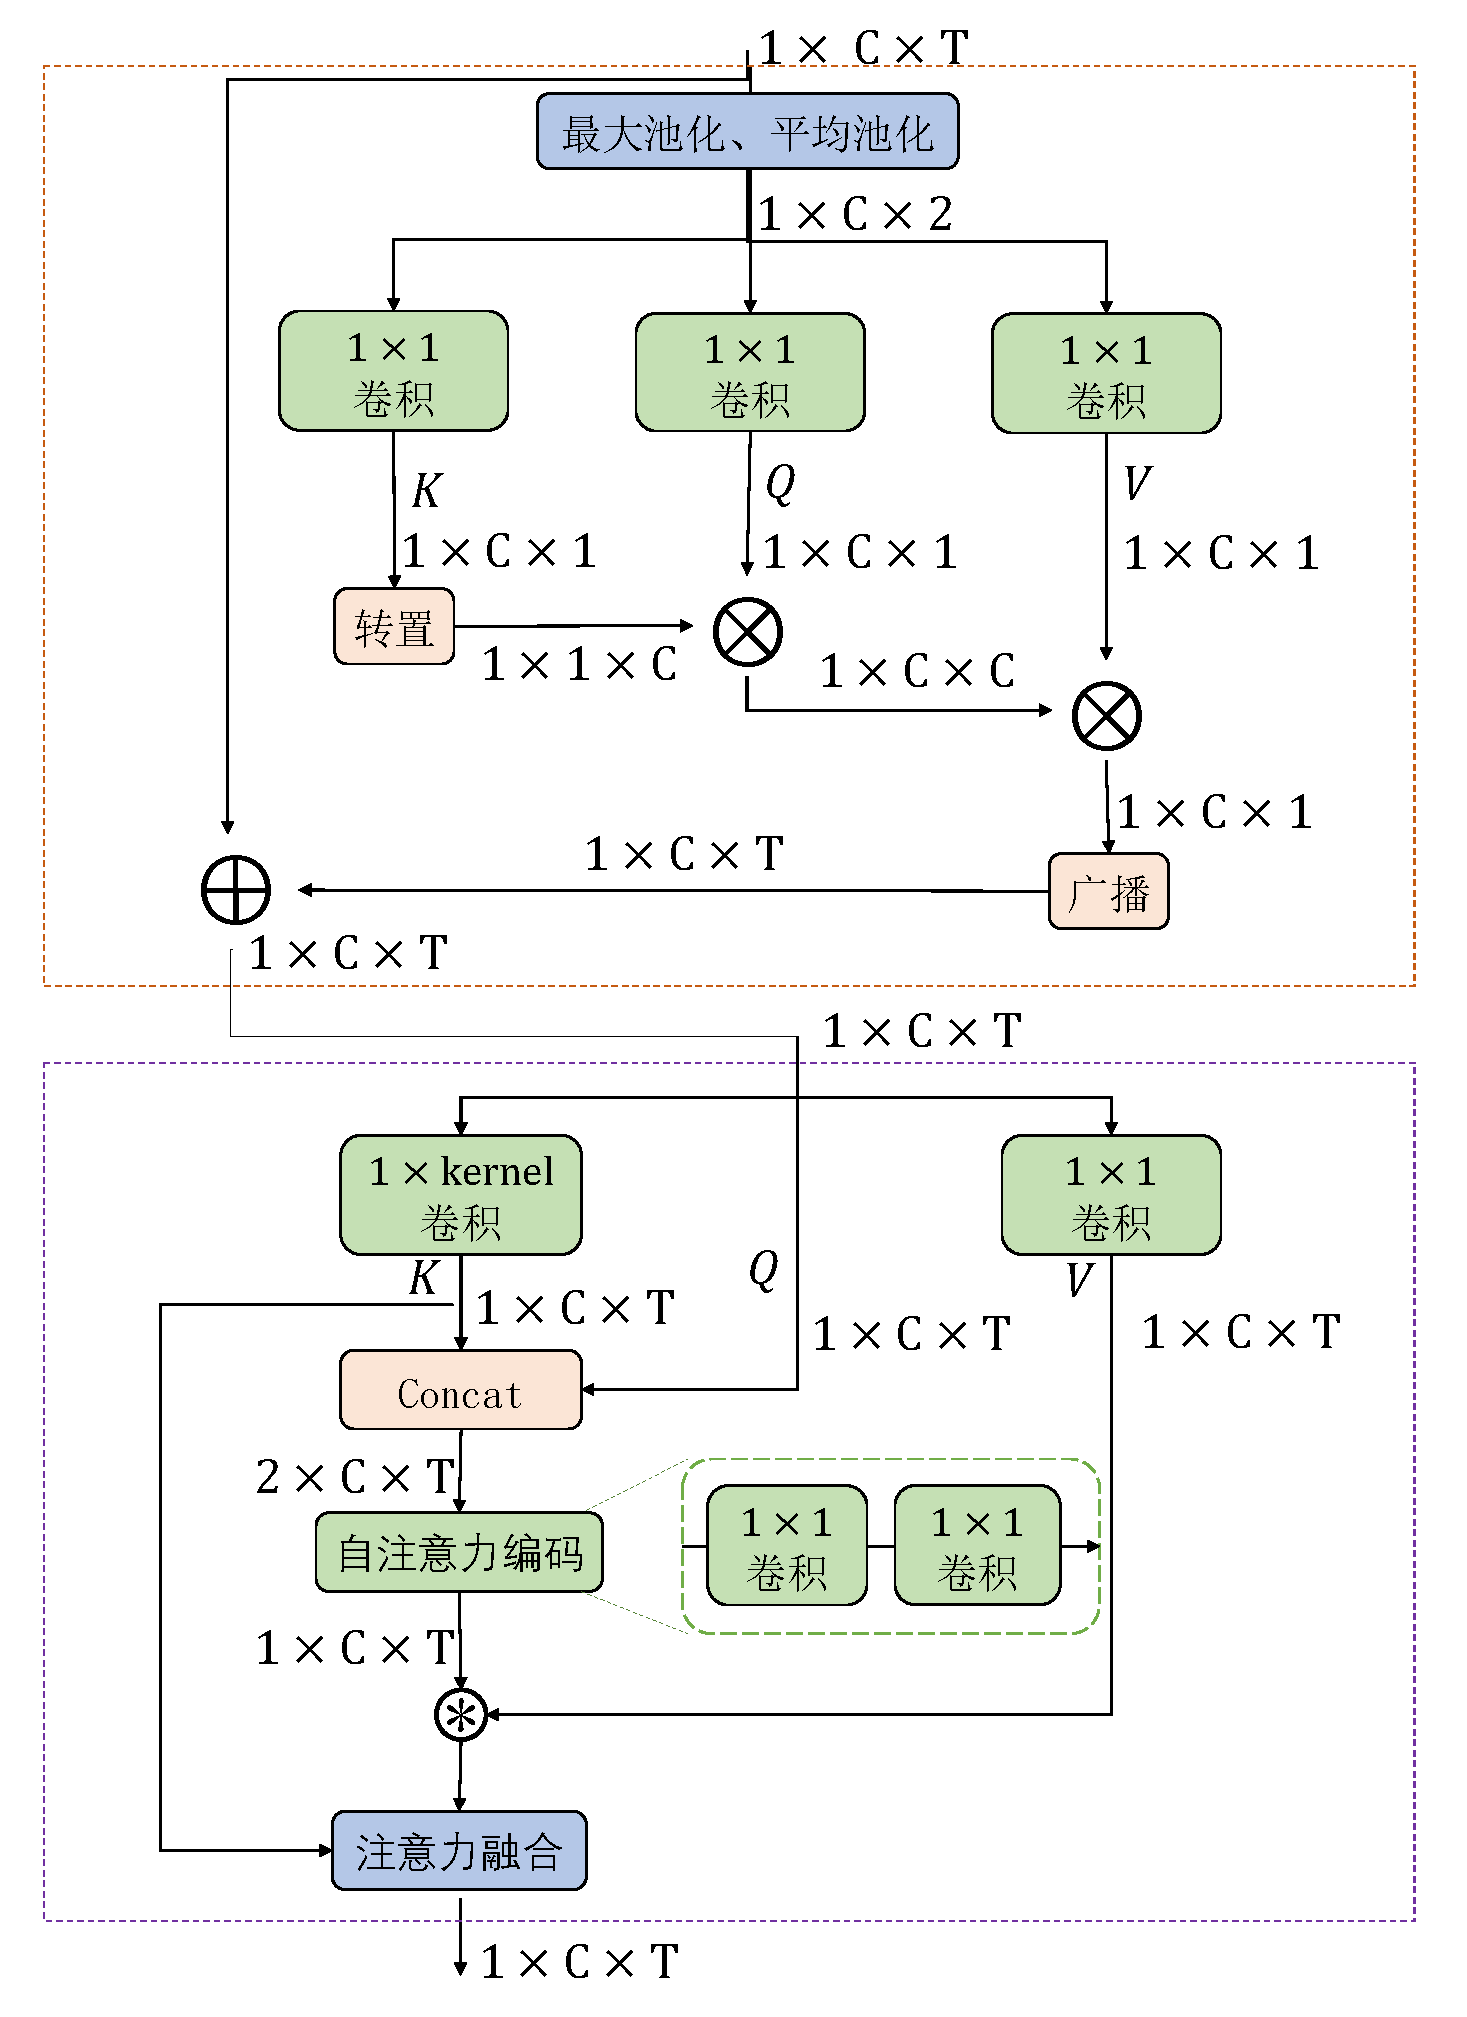
\includegraphics[width=0.5\textwidth]{gsa2.pdf}
    \caption{SCoT结构}
    \label{fig:gsa}
\end{figure}

SCoT分两个过程计算EEG信号的全局时空注意力,首先计算空域上的空间自注意力,使用空间自注意力对输入进行加权后,再基于加权数据计算时空域自注意力。空间自注意力能够为重要的电极(通道)分配更多的注意力,在局部相关性较弱的情况下突出不同通道的相对重要性。时空域自注意力能够充分利用时间序列数据中的局部相关性,以及已经由空间自注意力加权强化过的空间特征信息,从而更加精细而全面地捕获EEG信号中的全局时空依赖关系,同时对上一步得到的注意力进行一定的校准。此外,两个过程的计算也有利于降低计算的复杂度。

SCoT模块计算注意力的整体流程如公式~\ref{eq:scot}~所示。
\begin{equation}
    SCoT(X)=Att_{st}(Att_s(X)), \; X \in \mathbb{R}^{1 \times C \times T}
    \label{eq:scot}
\end{equation}
其中,\(X\)为EEG信号输入,\(C\)为通道,\(T\)为时间,\(Att_s\)为空间自注意力模块,\(Att_{st}\)为时空自注意力模块。

在空间自注意力模块中,首先进行混合池化操作,对输入进行转换,如公式~\ref{eq:scots1}~所示。
\begin{equation}
    X'=Concat[MaxPool(X),AvgPool(X)],\;X' \in \mathbb{R}^{2 \times C \times T}
    \label{eq:scots1}
\end{equation}

EEG信号具有低信噪比的特性,混杂了大量的噪声和干扰成分,通过结合最大池化操作和平均池化这两种操作,能够在最大程度保留EEG信号中关键特征的同时,对噪声起到一定的抑制作用,从而在不同的特征信息之间取得平衡。在取得池化表示\(X'\)后,通过公式~\ref{eq:scots2}~获得键、查询、值矩阵\(K\)、\(Q\)和\(V\)。
\begin{equation}\label{eq:scots2}
    K=X'W_K,\;Q=X'W_Q,\;V=X'W_V
\end{equation}
其中,\(W_K,\,W_Q,\,W_V\)分别是对应的权重参数,通过\(1\times1\)卷积获得。

随后,将\(K\)经过转置后与\(Q\)相乘,提取其相似性特征,并使用Softmax进行归一化,得到权重矩阵\(A\),得到的计算过程如公式~\ref{eq:scots3}~所示。
\begin{equation}\label{eq:scots3}
    A=Softmax(Q \bigotimes K^T),\;A \in \mathbb{R}^{1 \times C \times C}
\end{equation}
其中,\(\bigotimes\)代表克罗内克积。

\(A\)随后与值矩阵\(V\)相乘,实现对特征图的加权,并通过广播方式扩展到与输入特征图相同的尺寸,与输入特征图\(X\)加和后得到空间自注意力的输出,计算过程如公式~\ref{eq:scots4}~所示。
\begin{equation}\label{eq:scots4}
    Att_s(X)=X+Expand(A \bigotimes V)
\end{equation}

空间自注意力的输出被作为时空域自注意力模块的输入,以在时空域中利用经过强化的空间特征。首先通过\(1 \times kernel\)卷积提取时间域上的局部上下文特征,使得生成的键矩阵\(K\)具有输入特征图的静态上下文信息,对查询矩阵\(Q\)不做变换,使用\(1\times1\)矩阵获取值矩阵\(V\)。对于经过空间自注意力加权后的输出\(Y  \in \mathbb{R}^{1 \times C \times T}\),三个矩阵的计算过程如公式~\ref{eq:scotst1}~所示。
\begin{equation}\label{eq:scotst1}
    K=YW_K,\;Q=Y,\;V=YW_V
\end{equation}
其中,\(W_K,\,W_V\)分别是键矩阵和值矩阵对应的权重参数,在计算上,使用卷积进行获取,其过程如公式~\ref{eq:scotst2}~所示。
\begin{equation}\label{eq:scotst2}
    W_K=Conv_{1 \times kernel}(Y),\;W_V=Conv_{1 \times 1}(Y),\;kernel=\left \lfloor \frac{sfreq}{4} \right \rfloor 
\end{equation}
其中,\(kernel\)的值取决于采样率\(sfreq\),在此设定为\(\left \lfloor \frac{sfreq}{4} \right \rfloor\),是为了捕获4Hz以上的频率信号。

随后,\(K\)和\(Q\)在深度维度进行聚合,提取其相似度特征,并与\(V\)矩阵进行融合,获取特征图的动态上下文信息\(L\),其计算过程如公式\ref{eq:scotst3}~所示。
\begin{equation}\label{eq:scotst3}
    L=Fusion(V ,\, (Conv_{1 \times 1}(Conv_{1 \times 1}(Concat[K,Q])))),\;L \in \mathbb{R}^{1 \times C \times T}
\end{equation}
其中,\(\odot\)表示逐元素相乘的Hadamard乘法。通过两个\(1 \times 1\)卷积进行自注意力编码运算,学习动态多头注意力矩阵。\(Fusion\)为局部矩阵乘法运算,用于度量局部网格中每个query与相应key之间的成对关系,在计算上,公式~\ref{eq:scotst4}~表示了\(Fusion\)运算的集合,在时间域和空间域分别使用轴向卷积进行了局部矩阵乘法运算,随后进行了\(BN\)批量归一化和\(Softmax\)归一化。
\begin{equation}\label{eq:scotst4}
    Fusion=Conv_{channels \times 1}+Conv_{1 \times kernel} + BN + Softmax
\end{equation}

最后,将输入特征\(Y\)与\(L\)进行融合,得到时空域自注意力模块的输出\(Att_{st}\),如公式~\ref{eq:scotst4}~所示。融合方式参考了Transformer的残差连接思想,将\(Y\)与\(L\)经过Concat聚合之后由卷积进行融合,从而实现对特征的校准,最后,通过逐元素相乘得到校准后的加权输出。计算期间,对数据进行了多项变形(Reshape)操作。
\begin{equation}\label{eq:scotst5}
    Att_{st}=Softmax(Conv_{1 \times 1}(AvgPool(Concat[Y,L]))) \odot Y
\end{equation}

对运动想象脑电图分类任务来说,传统的全局自注意力机制忽视了EEG信号时域与空域的低局部相关性,导致网络无法很好对重要数据进行关注。SCoT通过两个过程进行全局时空注意力的提取,对EEG信号具有更好的适应性,同时降低了计算的复杂度。空间全局自注意力能够突出不同通道数据的重要性,为时空域的全局自注意力提供先验信息,时空域的全局自注意力利用时间域的局部上下文信息和轴向卷积,将输入特征图的静态上下文和动态上下文进行结合,能够增强输出特征图的表征能力。

\subsection{基于LSTM和SCoT的分类网络LS-Net}

长短期记忆网络属于循环神经网络,能够利用当前时间步及其之前的信息,并且解决了RNN在处理长期依赖问题时存在的梯度消失和梯度爆炸问题。LSTM通过单元状态存储和更新信息,使得模型能够记住历史信息,并且有选择地进行遗忘或者更新;通过门控机制(输入门、遗忘门、输出门),LSTM能够对信息的流动进行有效的控制,从而保留和传递长距离信息,提升对长期依赖关系的建模能力。考虑到LSTM具有出色的对时序数据进行建模的能力,论文选择使用LSTM来获取EEG信号中的时序长期依赖信息。

LSTM用于处理形状为\((sequence\_length,\, batch\_size,\, input\_size)\)的三维序列数据,其中\(sequence\_length\)为序列的长度,\(batch\_size\)为批量处理的样本数量,\(input\_size\)为每个时间步的特征维度。其输出同样是三维序列数据,形状与输入序列类似,具体为\((sequence\_length,\,batch\_size,\, hidden\_size)\),其中,\(hidden\_size\)为LSTM内部的隐藏维度。LSTM由一系列元胞连接而成,这些元胞按时间顺序逐个处理输入序列,在每一个时间步内,LSTM元胞进行以下操作:计算当前时间步的输入允许计入单元状态的程度;判断单元状态中应当被丢弃的信息;计算候选单元状态;更新单元状态;生成当前时间步的隐藏状态,以及将隐藏状态传递给下一个时间步或输出。

EEG信号是使用脑电采集设备采集的大脑在一段时间内的电压变化,天然具有时序属性,原始EEG信号为时间和通道的二维数据,其中,时间维度可以对应LSTM输入的序列长度,通道维度可以对应LSTM输入的特征维度。由此,可以将EEG信号以\((time\_samples,\, batch\_size,\, channels)\)的形式与LSTM的输入对齐,即将通道维度视为对应时间步(采样点)上数据所具有的特征。

虽然LSTM通过其内部的单元状态和门控结构缓解了RNN中存在的长期依赖的问题,但在处理较长的时间序列数据时,其性能仍存在局限性。LSTM在遍历时间序列的过程中,对每个时间步的输入信息均采用统一的方式通过隐藏状态进行累积和更新,并不具备针对当前任务为各个时间步的输入赋予不同重要性的能力。因此,有必要在LSTM模型中引入全局时空注意力机制SCoT模块,使得模型能够动态地对EEG信号中的重要数据进行关注,理解不同位置之间的深层次依赖关系,捕获更为完整的长距离信息,从而获得更为精确和全面的特征表示,提升模型处理EEG信号分类任务时的性能和泛化能力。

LSTM结合SCoT得到的网络结构如图~\ref{fig:ls}~所示,将其称之为LS-Net(LSTM-SCoT Net)。
\begin{figure}[ht]
    \centering
    \includegraphics[width=0.8\textwidth]{ls-net中.pdf}
    \caption{LS-Net结构}
    \label{fig:ls}
\end{figure}

LS-Net的输入为\(X \in \mathbb{R}^{C \times T}\),其中,\(C\)为通道数量,表示每个时间采样点所具有的特征数,\(T\)为时间,表示表示时间轴上的采样点序列长度。
在处理过程中,LSTM按时间序列递进地对每个采样点进行加工,LSTM的每个层(Layer)的输出结果为\(Y \in \mathbb{R}^{H \times T}\),其中,\(H\)为隐藏层数量。
在经过每个Layer处理后,\(Y\)由SCoT模块计算全局时空自注意力。需要说明的是,尽管\(H\)来自于LSTM的隐藏层维度,但在SCoT模块中,仍然将其视为通道维度特征进行处理,以对来自LSTM输出的特征进行整合,从而提升网络捕捉输入EEG信号全局时空依赖关系的能力。

\section{基于特征融合改进的分类网络}

为了综合LS-Net和DIS-Net的优点,论文选择以并行分支的形式将LS-Net引入DIS-Net网络结构中。这是因为直接以串联形式加入LS-Net可能导致模型仅能捕捉到经过深层卷积获得的特征图的依赖关系,而非充分利用全局信息。并行分支的设计旨在全面利用LS-Net对全局依赖的建模能力,同时避免干扰卷积神经网络本身的局部特征提取功能。

将LS-Net模块引入DIS-Net后获得的新模型命名为HA-FuseNet,其结构如图~\ref{fig:hafuse}~所示。

为了整合DIS-Net与LS-Net所提取的特征信息,将二者获取的特征图在深度维度进行特征聚合。为了确保两个分支的数据能够聚合,需要对数据形状进行适配处理。此外,由于需要使用历史信息,LSTM无法进行并行计算,因此同样需要对输入LSTM的数据进行一定的处理,以对计算效率进行平衡。

论文设计了C2R-Block和R2C-Block两种模块,用于并行分支间的交互融合。在C2R-Block中,对数据执行时间维度的卷积操作以实现下采样,将原始样本 \(X \in \mathbb{R}^{C \times T}\) 在时间轴上进行压缩,转化为 \(X' \in \mathbb{R}^{C \times T'}\) ,其中, \(C\) 代表通道数(电极数), \(T\) 代表原始时间序列长度,\(T'\)则代表下采样后的时间序列长度。另一方面,在R2C-Block中,采用反卷积技术对LS-Net模块产生的输出进行时间维度上的上采样,使其与DIS-Net分支的数据维度相符。最后,在深度维度对经过上述处理的两类特征进行聚合,从而充分融合卷积神经网络捕获的局部特征信息,以及长短期记忆网络揭示的时序依赖特性、全局自注意力模块发掘的全局时空依赖关系,以期全面提升模型对EEG信号的综合理解与分析能力。

\section{基于GhostNet改进的网络轻量化}

考虑到BCI系统对即时响应具有较高的要求,虽然HA-FuseNet通过轴向卷积和深度可分离卷积削减了一定的模型参数量和计算量,但为了追求更加卓越的实时性能表现,仍有进行进一步轻量化的必要。HA-FuseNet模型的参数主要来源于密集连接模块、长短期记忆网络和全局自注意力。针对长短期记忆网络和全局自注意力,论文通过下采样削减了输入数据的规模。与此同时,对于密集连接模块以及其他卷积层,论文进行针对性的轻量化卷积设计,并将在下文中对轻量化卷积模块的设计思路与方案加以阐述。

\subsection{基础轻量级网络结构}

MobileNet\cite{howard2017mobilenets}由Google团队提出,其核心思想在于引入了深度可分离卷积(Depthwise Separable Convolution),通过深度卷积处理单个输入通道,然后使用点积卷积(也称为逐点卷积或\(1 \times 1\)卷积)跨通道整合信息。这种分解大幅减少了计算成本和模型大小,同时保持了较高的精度。

ShuffleNet\cite{ma2018shufflenet}由旷视科技的研究团队所开发,其设计目标在于实现模型计算效率与预测准确性的均衡优化。ShuffleNet将输入特征图均匀划分为两个部分,一部分不经额外计算直接向下传输,另一部分则经历一系列计算后再与前者合并。二者在Concatenate操作之后,实施通道混洗操作,从而有效提升模型在轻量化条件下的性能表现。

GhostNet\cite{han2020ghostnet}由华为诺亚方舟实验室提出,其核心思想在于提出了幻影模块(Ghost Module),该模块针对深度神经网络中存在的潜在冗余和相关性较高的特征图问题,通过高效的计算策略提炼出“幻影特征图”。研究团队发现,在许多情况下,多个特征图可能蕴含着相似的模式信息,这意味着部分特征图的信息实质上可以从其他特征图中推衍得出,犹如“幻影”。鉴于此,GhostNet摒弃了对每组特征图均采用标准卷积的传统做法,转而采用一种更为经济高效的计算方式去合成这类“幻影特征图”。在具体实施中,首先运用有限数量的标准卷积层提取基础特征图,以此严格控制参数规模,接下来通过对基础特征图施加一组线性变换,高效地生成大量辅助特征图,这些辅助特征图被视为原始特征图的“幻影”。最后,Ghost模块将“幻影特征图”与标准卷积产生的少量核心特征图整合在一起,以有效模拟传统卷积所带来的丰富表征能力,在保持高精度的同时,降低了模型的计算复杂性和参数规模。Ghost模块的结构如图~\ref{fig:ghost}~所示,其中,Identity操作由标准卷积生成的特征图,\(\Phi\) 为廉价线性变换。
\begin{figure}[ht]
  \centering
  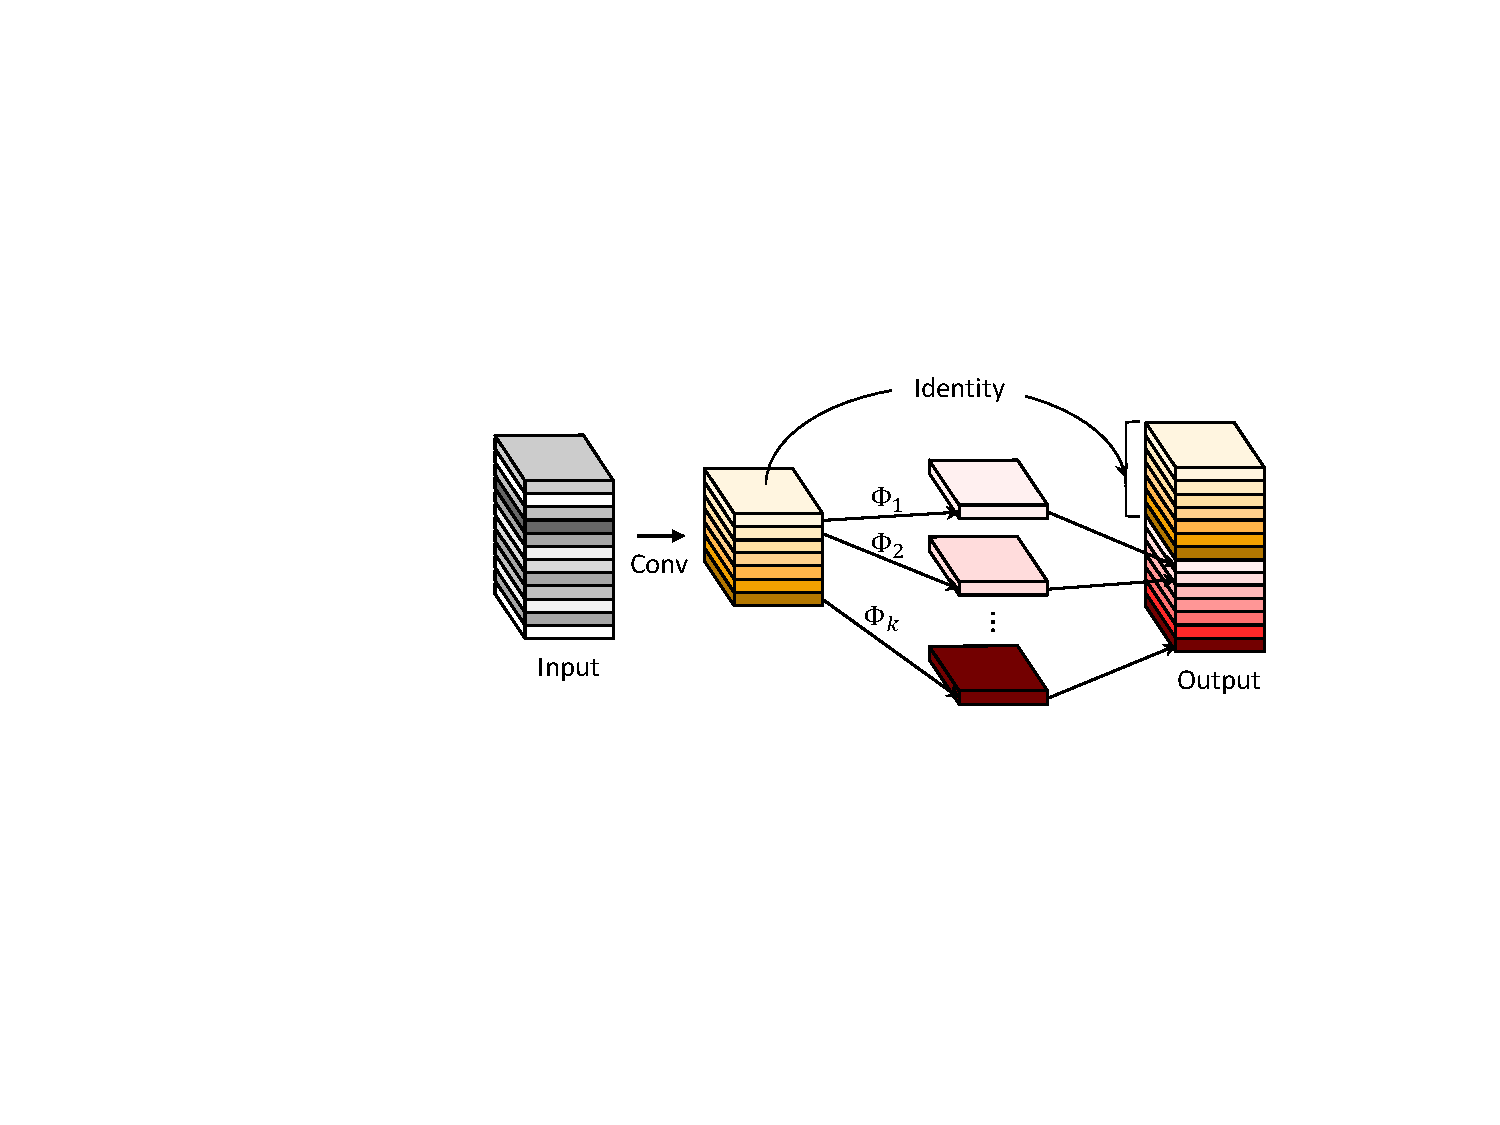
\includegraphics[width=0.6\textwidth]{ghost.pdf}
  \caption{Ghost模块结构\cite{han2020ghostnet}}
  \label{fig:ghost}
\end{figure}

\subsection{GhostNet结合MobileNet改进的轻量化卷积模块}

在HA-FuseNet架构中,已经通过轴向卷积削减了一定的模型参数量。因此,本节在现有成果的基础上,主要结合MobileNet和GhostNet所提出的Ghost模块进行了针对性改良。

GhostNet的优势在于其Ghost模块设计,该模块凭借对特征图间内在相似性的有效利用,实现了低成本的特征转换操作,同时,GhostNet中使用了权重参数 \(ratio\),用以控制经由廉价线性转换进行操作的特征图的比例,其中,使用标准卷积的生成的特征图数量为\(D_{out} \times ratio\),其中,\(D_{out}\)为输出特征图数量,使用可分离卷积的分支生成的特征图数量为\(D_{out}-D_{out} \times ratio\)。

然而,Ghost模块在运用线性变换与传统卷积相结合的方式来产生新特征图的过程中,尚存在一定的局限性:在深度可分离卷积的实现上,Ghost模块使用一层分组卷积对输入特征图进行转换,缺乏不同特征图之间的相互关系。因此,论文对Ghost模块进行了优化,使用更为标准的深度可分离卷积进行特征图的转换,构建出SG模块(Separable Ghost Module)。SG模块的结构如图~\ref{fig:sg}~所示,通过两层卷积(可分离卷积和点积卷积)增强不同特征图之间的相互作用,进而提升网络的整体表现力和特征学习能力。途中蓝色虚线框所包括的部分为替代原本卷积层的改动,\(D_{in}\)为输入特征图数量,\(D_{out}\)为输出特征图数量,\(ratio\)为权重参数。
\begin{figure}[ht]
    \centering
    \includegraphics[width=0.4\textwidth]{SG中2.pdf}
    \caption{SG模块结构}
    \label{fig:sg}
\end{figure}

对于SG模块,论文对廉价变换卷积层做了如下改进:根据采样频率特性调整卷积核大小,为了描述的简洁性,以时间域特征提取卷积模块为例,并将其卷积核大小设定为\(1 \times 25\),对于采样频率为250Hz的BCI Competition IV Dataset 2A数据集而言,意味着该卷积核以0.1秒的时间窗口进行特征捕获。在廉价变换卷积层,特征图首先以\(1 \times 25\)可分离卷积进行特征提取,不改变特征图数量;随后经过批归一化层,使用\(1 \times 1\)逐点卷积进行特征图之间的交互,改变特征图数量;最后,经过批归一化层与GELU激活函数。

廉价变换卷积层的输入特征图数量为\(D_{out} \times ratio\),输出特征图数量为\(D_{out}-D_{out} \times ratio\),以保证输出特征图数量无偏差,由标准卷积直接传递而来的输出特征图数量为\(D_{out} \times ratio\),所有特征图在深度维度进行聚合,获得最终的输出。

\section{本章小结}

本章主要对论文所提出的最终模型HA-FuseNet进行了详细的介绍。首先,针对运动想象脑电图分类领域现有方法中仍然存在的问题展开讨论和分析,并介绍了论文提出的最终模型HA-FuseNet的总体网络结构,同时,对HA-FuseNet的构建思路进行了简要的介绍。其次,详细阐述了HA-FuseNet的各个改进点。HA-FuseNet基于特征融合与注意力机制构建,包括DIS-Net和LS-Net两个子网络。DIS-Net基于多尺度密集连接与混合注意力机制对局部特征进行提取。LS-Net针对卷积神经网络局部特征提取的局限性,提出了LSTM结合全局自注意力模块SCoT的方式,LSTM具有提取长短期依赖的能力,SCoT模块采用两阶段计算的方式获取空间域和时空域的全局自注意力,从而在减少计算消耗的同时,获得更全面且有针对性的特征表达。将全局特征与局部特征进行深度维度的聚合,从而在避免特征相互干扰的情况下对不同的特征进行利用,得到更精准的分类效果。最后,介绍了HA-FuseNet的轻量化结构,从而更进一步对计算开销进行削减。